\begin{figure}[p!]
    \resizebox{\linewidth}{!}{
        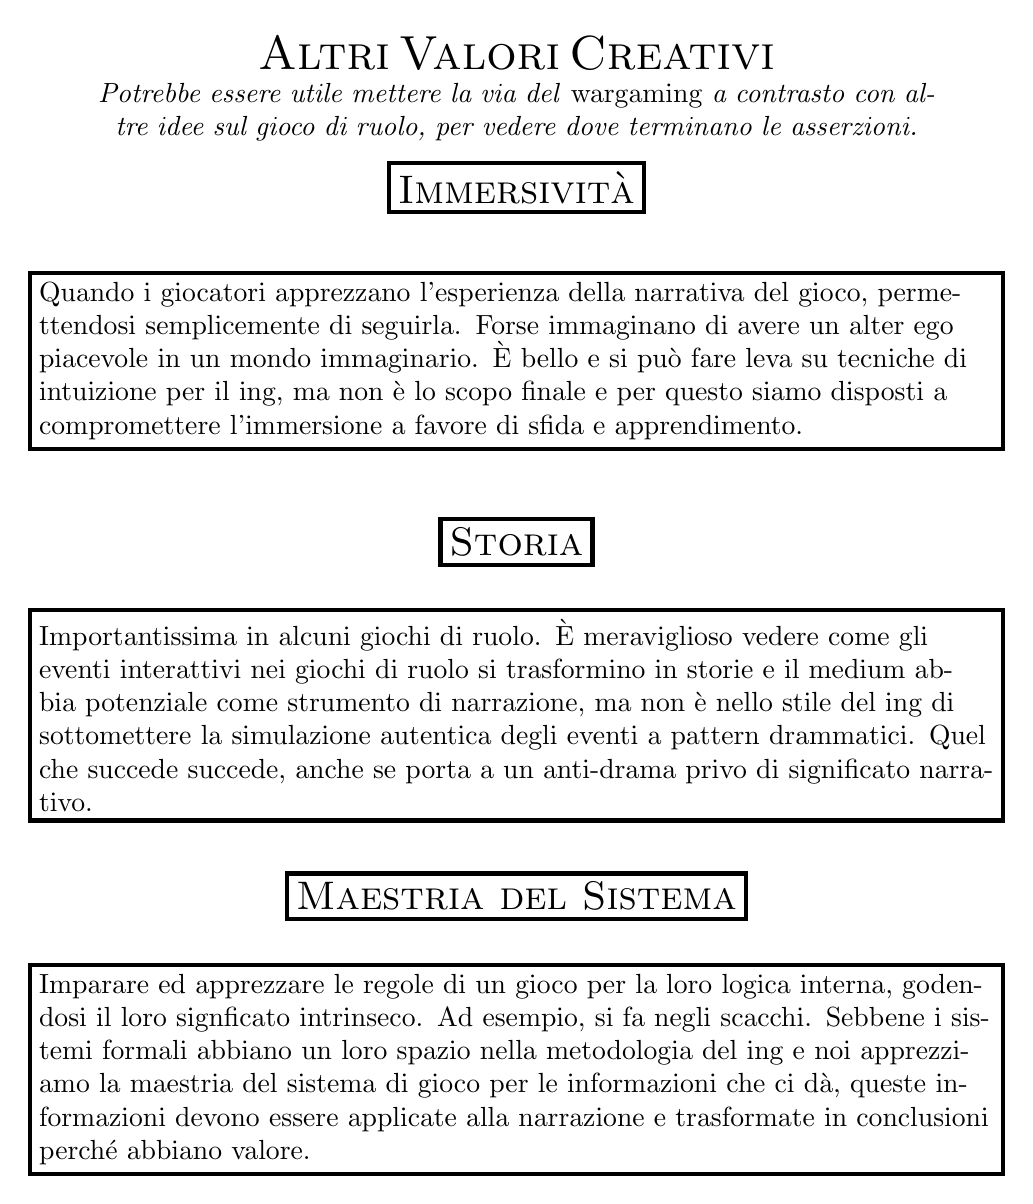
\begin{tikzpicture}
            \node[text width=\linewidth, align=center] (T) at (-1, 0.25) {
                    \textsc{\LARGE{Altri Valori Creativi}}\\
                    \textit{Potrebbe essere utile mettere la via del} wargaming \textit{a contrasto con altre idee sul gioco di ruolo, per vedere dove terminano le asserzioni.}
                };

            \node[draw, ultra thick, rectangle,font=\Large\scshape] (A) at (-1, -1) {Immersività};
            \node[draw, ultra thick, rectangle, text width=\linewidth] at (-1, -3.2) {
                Quando i giocatori apprezzano l'esperienza della narrativa del gioco, permettendosi semplicemente di seguirla. Forse immaginano di avere un alter ego piacevole in un mondo immaginario. È bello e si può fare leva su tecniche di intuizione per il \wargam{ing}, ma non è lo scopo finale e per questo siamo disposti a compromettere l'immersione a favore di sfida e apprendimento.
            };

            \node[draw, ultra thick, rectangle,font=\Large\scshape] (A) at (-1, -5.5) {Storia};
            \node[draw, ultra thick, rectangle, text width=\linewidth] at (-1, -7.7) {
                Importantissima in alcuni giochi di ruolo. È meraviglioso vedere come gli eventi interattivi nei giochi di ruolo si trasformino in storie e il medium abbia potenziale come strumento di narrazione, ma non è nello stile del \wargam{ing} di sottomettere la simulazione autentica degli eventi a pattern drammatici. Quel che succede succede, anche se porta a un anti-drama privo di significato narrativo.
            };

            \node[draw, ultra thick, rectangle,font=\Large\scshape] (A) at (-1, -10) {Maestria del Sistema};
            \node[draw, ultra thick, rectangle, text width=\linewidth] at (-1, -12.2) {
                Imparare ed apprezzare le regole di un gioco per la loro logica interna, godendosi il loro signficato intrinseco. Ad esempio, si fa negli scacchi. Sebbene i sistemi formali abbiano un loro spazio nella metodologia del \wargam{ing} e noi apprezziamo la maestria del sistema di gioco per le informazioni che ci dà, queste informazioni devono essere applicate alla narrazione e trasformate in conclusioni perché abbiano valore.
            };
            
        \end{tikzpicture}
    }
\end{figure}